%% KDD 2027 Datasets & Benchmarks (Cycle 1) — v2b-syndata
%% First draft: unconstrained length; 8-page trim happens per docs/KDD_SUBMISSION_PLAN.md WS-G.
%% Numbers marked \owed{...} await docs/experiments/PAPER_NUMBERS.md (WS-F); do not hand-edit them in.
\documentclass[sigconf,natbib=true]{acmart}

\usepackage{booktabs}
\usepackage{amsmath}
\usepackage{amssymb}

%% --- venue block (Cycle 1; update rightsretained per ACM form on acceptance) ---
\setcopyright{rightsretained}
\acmConference[KDD '27]{Proceedings of the 33rd ACM SIGKDD Conference on
  Knowledge Discovery and Data Mining}{August 2027}{TBD}
\acmBooktitle{Proceedings of the 33rd ACM SIGKDD Conference on Knowledge
  Discovery and Data Mining (KDD '27)}

%% --- notation macros (single source of truth; see KDD_PAPER_STRUCTURE.md) ---
\newcommand{\phifreq}{\phi}          % plug-in frequency
\newcommand{\kapcons}{\kappa}        % timing consistency
\newcommand{\deldist}{\delta}        % daily distance (km)
\newcommand{\ks}{\mathrm{KS}}
\newcommand{\wone}{W_1}
\newcommand{\cvrmse}{\mathrm{CV(RMSE)}}
\newcommand{\nmbe}{\mathrm{NMBE}}
\newcommand{\tstr}{\mathrm{TSTR}}
\newcommand{\trtr}{\mathrm{TRTR}}
\newcommand{\generator}{\textsc{v2b-syndata}}
%% sprint-owed numbers — grep for \owed before submission; must be zero hits
\newcommand{\owed}[1]{\textcolor{red}{$\langle$#1$\rangle$}}

\begin{document}

\title{\generator{}: A Calibrated, Reproducible Generator for
Vehicle-to-Building Energy Datasets}

%% Single-blind: real author block (fill before submission)
\author{Rishav Sen}
\affiliation{%
  \institution{Vanderbilt University}
  \city{Nashville}\state{TN}\country{USA}}
\email{rishav.sen@vanderbilt.edu}
%% TODO: co-authors + order

\begin{abstract}
Research on vehicle-to-building (V2B) coordination requires datasets that
couple building electrical load, electric-vehicle (EV) charging sessions,
driver behavior, electricity tariffs, demand-response (DR) events, and
distributed energy resources on a common clock. Such data is largely
unavailable: real charging logs are privacy-restricted and confined to a small
number of sites, and no charging equipment records battery state of charge
(SoC), the quantity most V2B optimization methods schedule around. We present
\generator{}, a configurable generator that produces coupled fifteen-minute
V2B datasets for parameterized scenarios under three guarantees. First, the
building load is \emph{physically simulated}: each dataset is produced by an
EnergyPlus simulation of a DOE prototype building under a perturbed
typical-year weather realization, and the same weather drives the photovoltaic
model and is exported alongside the data. Second, driver behavior is
\emph{calibrated}: arrival, dwell, and energy-demand distributions are fitted
per behavioral region from three real charging corpora---ACN-Data, EV~WATTS,
and ElaadNL---with fit quality and provenance recorded on every value; SoC
channels are explicitly modeled priors made consistent with observed energy,
never presented as measurements. Third, generation is \emph{reproducible}: a
scenario configuration and a single integer seed regenerate any dataset
bitwise, and every run emits a provenance manifest. We quantify
representativeness against real data (ASHRAE Guideline~14 building-load
fidelity versus ComStock and the Building Data Genome~2 meters; held-out,
confidence-interval-quantified distributional fidelity versus the calibration
corpora) and demonstrate utility with train-on-synthetic/test-on-real
forecasting that performs on par with training on real data
(\tstr{}/\trtr{} MAE ratio $0.99$ on ACN-Data), together with a cross-cohort
transfer study. We release the generator (MIT), datasets (CC~BY~4.0),
Croissant metadata, a datasheet, sixty benchmark scenario configurations, and
an 18{,}000-sample ten-building reference corpus.

\end{abstract}

\begin{CCSXML}
<ccs2012>
<concept>
<concept_id>10002951.10003227.10003351</concept_id>
<concept_desc>Information systems~Data mining</concept_desc>
<concept_significance>300</concept_significance>
</concept>
<concept>
<concept_id>10010147.10010257.10010293.10010294</concept_id>
<concept_desc>Computing methodologies~Simulation types and techniques</concept_desc>
<concept_significance>500</concept_significance>
</concept>
<concept>
<concept_id>10010405.10010481.10010485</concept_id>
<concept_desc>Applied computing~Engineering</concept_desc>
<concept_significance>300</concept_significance>
</concept>
</ccs2012>
\end{CCSXML}
\ccsdesc[500]{Computing methodologies~Simulation types and techniques}
\ccsdesc[300]{Information systems~Data mining}

\keywords{synthetic data, data generator, electric vehicles,
vehicle-to-building, smart charging, building energy, calibration,
reproducibility, benchmark}

\maketitle

\section{Introduction}
\label{sec:intro}

Commercial buildings and workplace electric-vehicle (EV) fleets are converging
on a shared electrical envelope. When chargers are bidirectional, parked
vehicles become schedulable storage for the building---vehicle-to-building
(V2B) coordination---and the design questions multiply: how many chargers does
a site need, how much peak reduction can a fleet deliver, how should charging
be scheduled against a time-of-use tariff, and how do these answers change
with climate, building type, or workforce composition. Methods that answer
such questions, whether optimization-based or learned, must be developed and
evaluated on data that couples several channels at once: the building load,
the charging sessions, the drivers' arrival and departure behavior, the
tariff, demand-response (DR) events, and any on-site photovoltaics (PV) or
stationary storage, all on a common clock.

That data largely does not exist. Three barriers recur. First,
\emph{privacy}: charging records identify drivers and facilities, so
operational logs rarely leave the utility or campus that collected them.
Second, \emph{site lock-in}: the public exceptions---ACN-Data
\citep{lee2019acn}, ElaadNL open data \citep{elaadnl2020}, the EV~WATTS
evaluation dataset \citep{evwatts2023}---cover a handful of venues and fixed
infrastructures; one cannot ask a Pasadena workplace dataset how a Miami
retail site would behave, nor scale it to five hundred vehicles. Third, and
least appreciated, \emph{the key control variable is unmeasured}: charging
equipment meters energy, not batteries, so no public dataset records battery
state of charge (SoC)---the quantity nearly every V2B scheduling formulation
constrains and optimizes.

Synthetic generation addresses all three barriers if---and only if---the
generated data can be trusted. A generator provides privacy by construction,
supports counterfactual scenarios and arbitrary scale, and can label
quantities (such as SoC) that measurement cannot reach. The obligation this
creates is evidential: for a synthetic dataset to support methodological
conclusions, its \emph{representativeness} must be quantified against real
data and its \emph{utility} for downstream learning must be demonstrated
rather than asserted. These are precisely the criteria the KDD Datasets and
Benchmarks track sets for data generators, and they organize this paper.

We present \generator{}, a configurable generator of coupled V2B datasets. A
scenario is specified by five descriptors---site, building, driver population,
charging equipment, and measurement noise---and one integer seed; the
generator emits a coherent bundle of fifteen-minute time series and entity
tables: building load split into flexible and inflexible components, charging
sessions, driver and vehicle attributes, chargers, tariff prices, DR events,
PV generation, and storage specifications, together with a provenance
manifest. Three properties define the design.

\begin{itemize}
\item \textbf{Physical.} Building load is not a shape template: every dataset
is produced by an EnergyPlus \citep{crawley2001energyplus} simulation of an
ASHRAE 90.1-2019 DOE prototype building \citep{pnnl_prototypes} under
typical-meteorological-year weather subjected to a controlled, per-sample
perturbation. The identical perturbed weather frame drives the PVWatts-style
PV model \citep{dobos2014pvwatts} and is exported with the dataset, so load,
PV, and weather can never disagree.
\item \textbf{Calibrated.} Driver behavior is organized on three interpretable
axes---plug-in frequency $\phifreq$, timing consistency $\kapcons$, and daily
distance $\deldist$---partitioned into behavioral regions. Arrival, dwell, and
energy-requirement distributions are fitted per region by maximum likelihood
from three real charging corpora (ACN-Data, EV~WATTS, ElaadNL), with fit
quality (Kolmogorov--Smirnov distance) and provenance stamped on every fitted
value. Because no source measures SoC, the SoC channels are \emph{explicitly
modeled priors} reconstructed from delivered energy and inferred battery
capacity; we state this contract prominently rather than presenting modeled
values as measurements.
\item \textbf{Reproducible.} Randomness is drawn from hash-keyed substreams
(one per graph node, vehicle, and day), so a scenario configuration and one
seed regenerate any dataset bitwise, on any machine, regardless of the order
in which features were added to the generator. Every run records a manifest
containing each configuration value with its source, per-file checksums, and
the validation verdict.
\end{itemize}

\paragraph{Contributions.}
(i)~A forward-sampling generative model for coupled V2B data whose behavioral
layer is calibrated per region from three real charging corpora and whose
building layer is a real EnergyPlus simulation, with a single weather
realization shared by load, PV, and the exported weather channel
(\S\ref{sec:generator}--\S\ref{sec:calibration}).
(ii)~A reproducibility contract---order-independent hash-keyed randomness,
bitwise regeneration, per-value provenance manifests---accompanied by a
datasheet \citep{gebru2021datasheets}, Croissant metadata
\citep{akhtar2024croissant}, and dual licensing (\S\ref{sec:generator},
\S\ref{sec:release}).
(iii)~A two-sided evaluation meeting the generators bar: representativeness
via ASHRAE Guideline~14 building-load fidelity against ComStock
\citep{parker2023comstock} and Building Data Genome~2 \citep{miller2020bdg2}
meters, and held-out, confidence-interval-quantified distributional fidelity
against the calibration corpora (\S\ref{sec:representativeness}); utility via
train-on-synthetic/test-on-real forecasting at parity with training on real
data on ACN-Data, plus a cross-cohort transfer study
(\S\ref{sec:utility}).
(iv)~A released benchmark suite: sixty scenario configurations spanning nine
sites, six building types, thirteen driver cohorts, and six equipment mixes;
distribution-shift cohort pairs; and an 18{,}000-sample ten-building reference
corpus (\S\ref{sec:release}).

\section{Related Work}
\label{sec:related}

\paragraph{Real charging datasets.}
ACN-Data \citep{lee2019acn} remains the reference workplace-charging corpus:
per-session records from Caltech, JPL, and an office site, including
driver-entered energy requests. ElaadNL publishes anonymized public-charging
transactions from the Netherlands \citep{elaadnl2020}, and the DOE-funded
EV~WATTS program released a large multi-venue evaluation dataset
\citep{evwatts2023}. The INL EV Project \citep{inl2015evproject} documents an
earlier (2011--2013) residential fleet. These corpora anchor our calibration
(\S\ref{sec:calibration}); their limitations---few sites, fixed
infrastructure, no SoC channel, restricted or aggregated building-side
data---motivate generation rather than reuse.

\paragraph{Building-energy data and simulation.}
On the building side, large public resources exist: NREL's ComStock
\citep{parker2023comstock} provides calibrated end-use load profiles for the
U.S. commercial stock, and the Building Data Genome~2 project
\citep{miller2020bdg2} publishes meter data from over a thousand buildings.
Physics-based simulation via EnergyPlus \citep{crawley2001energyplus} with the
DOE prototype building models \citep{pnnl_prototypes} is the standard for
controlled building-load studies. We use simulation as the generative
mechanism and the public corpora as \emph{ground truth for validation}, which
keeps the two roles---generation and evaluation---separate by construction.

\paragraph{Synthetic EV-charging data.}
Session-level generative models appear in charging-infrastructure simulators:
ACN-Sim \citep{lee2021acnsim} includes generative session models fitted to
ACN-Data, and ElaadNL distributes simulation profiles derived from its
transactions. These target the charging channel in isolation. General-purpose
deep generative models for tabular and time-series data---GAN-based
\citep{yoon2019timegan,esteban2017rgan} and diffusion-based more
recently---can imitate a single site's joint distribution, but they offer no
scenario control (one cannot move the learned site to another climate or
double its fleet), no mechanism for physical consistency across coupled
channels, and no per-value auditability. \generator{} takes the opposite
trade: parametric distribution families joined by an explicit copula, fitted
per behavioral region, embedded in a physical simulation---less expressive
than a deep density model at any single site, but controllable, auditable,
physically coherent across channels, and calibrated across multiple corpora.
We quantify what this trade costs (and buys) in
\S\ref{sec:representativeness}--\S\ref{sec:utility}.

\paragraph{Evaluating synthetic data.}
We follow the two-sided evaluation that has become standard: distributional
fidelity against held-out real data, and downstream utility via
train-on-synthetic/test-on-real (TSTR) protocols introduced for medical
time series \citep{esteban2017rgan}. For building-load fidelity we adopt the
calibration metrics of ASHRAE Guideline~14 \citep{ashrae2014g14}
($\cvrmse{}$, $\nmbe{}$), which are the accepted standard for comparing
simulated to metered building energy. Documentation follows Datasheets for
Datasets \citep{gebru2021datasheets} and the Croissant machine-readable
metadata format \citep{akhtar2024croissant}.

\section{The Generator}
\label{sec:generator}

\generator{} is a forward-sampling generative model: a directed acyclic graph
(DAG) of samplers and renderers executed in topological order, in which every
random draw is taken from a named, seed-derived substream. This section
describes the layers in execution order; Figure~\ref{fig:pipeline} gives the
overview.

\begin{figure*}[t]
  \centering
  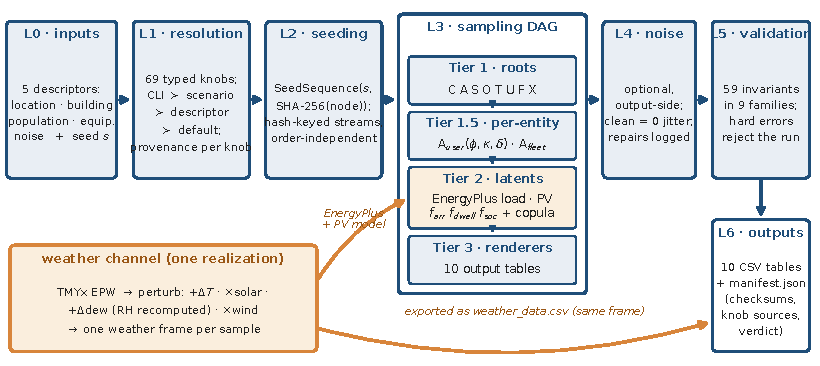
\includegraphics[width=\textwidth]{figures/fig1_pipeline.pdf}
  \caption{Pipeline overview. Five scenario descriptors and one seed resolve
  into a typed configuration; a sampling DAG produces latent variables and
  renders ten output tables; optional output-side noise, feasibility checks,
  and validation follow; a provenance manifest seals the run. A single
  perturbed weather realization (left) drives the building simulation, the PV
  model, and the exported weather channel.}
  \label{fig:pipeline}
\end{figure*}

\subsection{Scenario configuration and provenance}
\label{sec:knobs}

A scenario names five \emph{descriptors}---location, building, population,
equipment, and noise---each an entry in a small library, plus an optional set
of overrides. Descriptors expand into a flat namespace of 69 typed
configuration parameters (``knobs''), each with a declared type, range, and
default. Resolution follows a strict priority: command-line override
$\succ$ scenario override $\succ$ descriptor expansion $\succ$ registry
default. Every resolved value is stored with its source label (explicit,
descriptor, calibration provenance, or default), so the manifest of any
generated dataset answers, for all 69 parameters, \emph{why} each value is
what it is. Calibrated behavioral parameters
(\S\ref{sec:calibration}) enter through the same mechanism as
range-validated leaves carrying their calibration provenance; an out-of-range
override is rejected rather than clamped.

\subsection{Deterministic, order-independent randomness}
\label{sec:seeding}

All randomness derives from one integer seed $s$. Each DAG node $v$ draws from
a generator initialized with
$\mathrm{SeedSequence}(s,\ \mathrm{key}=h(v))$, where $h$ is a 32-bit digest
of the node \emph{name} (SHA-256 truncation); per-vehicle streams append the
vehicle index, and the session sampler keys additionally on the calendar day.
Because keys are content hashes rather than spawn order, adding a node to the
graph cannot shift any existing node's stream: datasets are bitwise
reproducible across generator versions that do not deliberately change a
sampler. Regression tests assert byte-identical output for fixed
$(\text{scenario}, s)$.

\subsection{Building load: simulated physics under controlled weather}
\label{sec:building}

The building channel is produced by EnergyPlus. The archetype and size
descriptors select an ASHRAE 90.1-2019 DOE prototype model (small, medium, or
large office; strip-mall or standalone retail; a mixed archetype averages an
office and a retail run). The location descriptor selects a
typical-meteorological-year (TMYx) weather file. Before simulation, the
weather is perturbed by four controlled channels: an additive dry-bulb offset
$\Delta T$, a multiplicative solar scale on the irradiance components, an
additive dew-point offset with relative humidity recomputed for thermodynamic
consistency (Magnus formula), and a multiplicative wind-speed scale. The
simulation runs at a fifteen-minute timestep and reports eight end-use meters,
which we aggregate into a \emph{flexible} component (cooling, heating, fans,
water systems---loads a building controller could in principle shift) and an
\emph{inflexible} component (interior and exterior lighting and plug loads).
Meter energies $E_J$ (joules per 900\,s interval) convert to mean interval
power as $P = E_J / (900 \times 1000)$~kW. A configuration switch either
normalizes the profile so that its peak equals the descriptor's design peak
(useful for controlled cross-scenario comparisons) or passes raw simulated
magnitudes through (used for all fidelity evaluation in
\S\ref{sec:representativeness}).

Two properties of this layer matter downstream. First, the \emph{same}
perturbed weather frame is consumed by the building simulation and the PV
model and is exported as the dataset's weather channel, so the released
channels are mutually consistent by construction. Second, weather perturbation
is \emph{input-side} variance: in multi-sample generation each sample draws
its own perturbation and is re-simulated, yielding physically faithful
sample-to-sample variability that cannot violate any downstream constraint.

\subsection{Drivers, vehicles, and charging sessions}
\label{sec:sessions}

\paragraph{Behavioral coordinates.}
Each driver is described by three axes: plug-in frequency
$\phifreq \in [0,1]$ (probability of appearing on a workday), timing
consistency $\kapcons \in [0,1]$, and daily distance $\deldist$ (km). A
\emph{population} is a weighted set of axis-aligned regions (boxes) in this
space. A driver is assigned a region categorically by weight, draws
$(\phifreq, \kapcons, \deldist)$ uniformly within the region's bounds, a
negotiation type from an empirical four-cluster mix, and a vehicle battery
class (24--100\,kWh) from the fleet mix.

\paragraph{Per-region distributions.}
Each region carries distribution parameters for arrival hour (truncated
normal, or a $k$-component truncated-normal mixture), dwell duration (Weibull,
or a two-component Weibull mixture), and the two SoC quantities (Beta
distributions), together with a Gaussian-copula correlation $\rho$ linking
arrival and dwell. When a population is calibrated
(\S\ref{sec:calibration}) these parameters are fitted values with recorded
provenance; hand-specified populations carry domain-informed values labeled
as such.

\paragraph{Session synthesis.}
For each vehicle and each eligible day, the vehicle appears with probability
$\phifreq$ (weekends scaled by a calibrated factor). On appearance, one joint
draw is made: a copula pair $(u_a, u_d)$ with correlation $\rho$ is
transformed through the inverse cumulative distribution functions of the
arrival and dwell marginals (mixtures are inverted by bisection on the
monotone mixture CDF, preserving the one-uniform-per-draw discipline that
determinism requires); arrival SoC and the required departure SoC are drawn
from their Beta marginals. The candidate session must then pass six
feasibility gates, evaluated atomically:
\begin{enumerate}
\item \emph{same-day}: departure falls on the arrival's calendar day;
\item \emph{window}: the session lies within the simulated horizon;
\item \emph{non-overlap}: arrival does not precede the vehicle's previous
  departure;
\item \emph{SoC monotonicity} (D6): required departure SoC strictly exceeds
  arrival SoC;
\item \emph{behavioral floor} (D7): required departure SoC meets the
  population's minimum-departure prior (active for hand-specified
  populations; calibrated cohorts set the floor to zero so fitted
  distributions are not clamped);
\item \emph{energy reachability} (D5):
  $\frac{(r - a)}{100}\,C \;\le\; P_{\max}\, \tau$,
  where $r$ and $a$ are required and arrival SoC (\%), $C$ the battery
  capacity (kWh), $P_{\max}$ the maximum charger rate (kW), and $\tau$ the
  dwell (h).
\end{enumerate}
A failed gate rejects the entire draw; after five rejections the vehicle-day
is dropped. Feasibility is thus enforced by \emph{rejection, never by
clamping}, so the emitted marginals are the fitted families conditioned on
feasibility rather than distorted by projection.

\subsection{Tariffs, demand response, PV, and storage}
\label{sec:der}

The tariff channel renders the location descriptor's rate structure (flat or
time-of-use with a peak window; a demand charge is carried as metadata for
downstream cost models). DR events are sampled from an inhomogeneous Poisson
process by thinning \citep{lewis1979thinning}: a base rate is modulated by
program season, weekday preference, a daily-maximum-temperature ramp driven
by the same weather realization, and a time-of-day window, then capped by
per-program monthly and seasonal limits; each program (CBP, BIP, ELRP)
carries its notification lead time. PV generation follows the PVWatts v5
chain \citep{dobos2014pvwatts}: plane-of-array irradiance by isotropic
transposition from the perturbed weather, cell temperature by the NOCT model,
temperature-derated DC power, and inverter-clipped AC power; the model is
deterministic, so PV varies across samples only through weather. Stationary
storage is released as a specification (capacity, power, efficiency, SoC
window)---deliberately without a dispatch schedule, since dispatch is a
decision of the downstream controller under evaluation, not exogenous data;
the same reasoning leaves charging \emph{schedules} out of the vehicle
tables.

\subsection{Output-side noise (optional)}
\label{sec:noise}

Separate from input-side weather variance, an optional noise layer perturbs
the \emph{rendered} tables to emulate measurement error: multiplicative
Gaussian jitter on load and prices, arrival-time jitter, arrival-SoC jitter,
and DR-notification dropout, in named profiles from ``clean'' (all zero; the
default, and the setting for every evaluation in this paper) to
``adversarial.'' Jitter can push a session past the sampler's feasibility
gates, so the layer re-clamps orderings and repairs reachability, recording
every repair in the manifest. Because repairs alter the guaranteed-feasible
contract, multi-sample corpora are generated with the clean profile and
input-side weather variance instead.

\subsection{Validation and the manifest}
\label{sec:validation}

Before a run is accepted, the generator checks the rendered tables against a
catalog of 59 invariants in nine families: schema, referential integrity,
temporal consistency (including same-day and non-overlap), SoC physics
(including reachability), charger conventions, behavioral-axis bounds,
CONSENT-share consistency, tariff and DR rules, and manifest integrity
(row counts and SHA-256 checksums). Charger-concurrency feasibility is
additionally measured and reported. The manifest records the full resolved
configuration with sources, generator version and git revision, per-file
checksums, feasibility metrics, any noise repairs, and the validation verdict
--- making every released file auditable and every run regenerable.

\section{Calibration from Real Charging Data}
\label{sec:calibration}

The behavioral layer is calibrated per region from real charging corpora. The
pipeline is: normalize a source corpus; summarize each real driver by the
axes $(\phifreq, \kapcons, \deldist)$; assign drivers to regions; fit each
region's distributions by maximum likelihood; and write the fitted parameters,
sample sizes, fit quality, and provenance back into the population library
that generation consumes.

\subsection{Sources}
\label{sec:sources}

Table~\ref{tab:sources} summarizes the corpora. Each source has its own
normalizer and its own region geometry: region boxes are anchored on each
corpus's empirical $(\phifreq,\kapcons)$ cloud rather than shared, so one
dataset's assumptions are not imposed on another. For ElaadNL this
re-anchoring reduced unassigned drivers from 76\% to 0\%; the ACN grid
predates the exercise and its re-anchoring is noted as future work
(\S\ref{sec:limitations}). The INL EV Project cohort is included as a
\emph{fixture-calibrated} legacy population: its parameters are hand-seeded to
the published fleet character (24\,kWh-era vehicles) rather than fitted from
raw records, and it is released---so labeled---as a distribution-shift
benchmark rather than claimed as a calibration corpus.

\begin{table}[t]
\caption{Calibration sources. ``Fitted'' populations carry per-region MLE
parameters with recorded provenance; the INL cohort is a labeled fixture.
\owed{Regenerate counts with WS-F; EV WATTS row from populations.yaml
metadata.}}
\label{tab:sources}
\centering\small
\begin{tabular}{@{}lllll@{}}
\toprule
Corpus & Span & Venue & Scale & Policy \\
\midrule
ACN-Data & 2019--21 & workplace (3 sites) & 632 users / 41{,}774 sessions & fitted \\
EV~WATTS & 2019--23 & workplace (public rel.) & 1{,}265{,}017 sessions & fitted \\
ElaadNL & 2020--24 & EU public & 55{,}379 sessions / 1{,}231 drivers & fitted \\
INL EVP & 2011--13 & residential & fixture (65 sessions) & fixture \\
\bottomrule
\end{tabular}
\end{table}

\subsection{Axes, regions, and assignment}

For each real driver we compute $\phifreq$ (share of active days with a
session), $\kapcons$ (timing consistency of arrivals), and $\deldist$ (a
distance proxy). Drivers fall into the first region box containing their
$(\phifreq,\kapcons)$; unassigned fractions are 0--0.5\% on the current grids.
Region \emph{weights} are the empirical user shares---for ACN:
rare-consistent 36.1\%, occasional-consistent 39.8\%, regular-charger 23.0\%,
rare-inconsistent 0.6\%---so the generated population reproduces the observed
cohort composition, not a designer's guess. The empirical geometry is itself
informative (Fig.~\ref{fig:axes}): real workplace drivers plug in far less
often than intuition suggests (76\% of ACN drivers at $\phifreq \le 0.3$),
which the calibrated grids encode and hand-authored grids would have missed.

\begin{figure}[t]
  \centering
  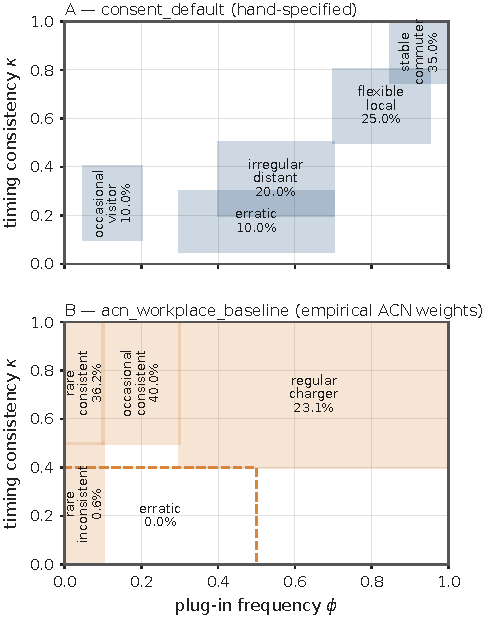
\includegraphics[width=\linewidth]{figures/fig2_axes.pdf}
  \caption{Region geometries in the $(\phifreq,\kapcons)$ plane. Top: the
  hand-specified \texttt{consent\_default} grid concentrates mass at high
  plug-in frequency. Bottom: the ACN-anchored grid, with empirical user-share
  weights, places 76\% of drivers at $\phifreq \le 0.3$; the dashed box is a
  region with zero empirical weight.}
  \label{fig:axes}
\end{figure}

\subsection{Per-region distribution fitting}

Within each region we fit: arrival hour by truncated-normal maximum likelihood
on a $[4,22]$\,h window, upgraded to a $k$-component mixture only when the
mixture improves the Kolmogorov--Smirnov distance by at least $0.02$; dwell by
Weibull MLE with the same mixture rule; and the arrival--dwell dependence by a
Gaussian copula with $\rho$ obtained from the Spearman rank correlation.
Mixture fits require at least 60 sessions and any fit at least 30; smaller
cells fall back to pooled fits. Fitting is per region rather than pooled: the
largest ACN region (rare-consistent, 36\% of drivers) arrives systematically
later than the pooled corpus, and replacing a broadcast pooled fit with its
own fit reduced its arrival KS from $0.179$ to $0.079$. The fitted arrival
distribution for that region is bimodal (morning and early-afternoon
components), a structure a single truncated normal cannot express
(Fig.~\ref{fig:arrival}).

\begin{figure}[t]
  \centering
  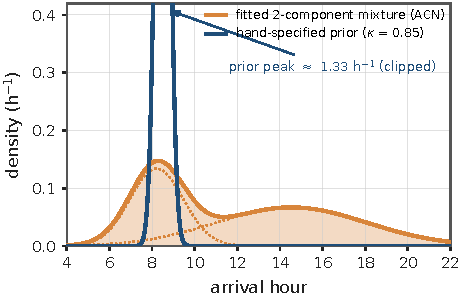
\includegraphics[width=\linewidth]{figures/fig3_arrival.pdf}
  \caption{Arrival-hour density for the largest ACN region: hand-specified
  prior (unimodal truncated normal) versus the fitted two-component mixture
  ($0.42\,\mathcal{N}(8.21, 1.25) + 0.58\,\mathcal{N}(14.54, 3.52)$, truncated
  to $[4,22]$\,h). Real workplace arrivals are bimodal.}
  \label{fig:arrival}
\end{figure}

\subsection{The SoC contract}
\label{sec:soc}

No public charging dataset records state of charge: equipment meters energy.
Both SoC channels are therefore \emph{modeled priors made consistent with
observed energy}, and we state the reconstruction explicitly. Arrival SoC is
drawn from a shared, seeded prior; the required departure SoC is calibrated
per region as the arrival prior plus delivered energy over inferred battery
capacity---delivered energy being the one universally recorded real signal.
Battery capacity is inferred per driver from maximum observed session energy,
falling back to vehicle-class defaults for roughly a third of ACN drivers.
Every SoC-related fitted value carries a provenance stamp identifying this
contract, and the datasheet repeats it. We regard the explicitness of this
contract as a feature of the release: downstream users can accept, replace,
or stress the prior, but cannot mistake it for measurement.

\section{Representativeness}
\label{sec:representativeness}

The generators category requires representativeness to be quantified. We
evaluate the building channel against independent real meter corpora, the
behavioral channel against the calibration corpora under a held-out protocol
with bootstrap confidence intervals, and the DER channels against an external
reference implementation. All evaluations use the clean noise profile and raw
(non-peak-normalized) simulated magnitudes.

\subsection{Building load versus real meters}
\label{sec:loadfidelity}

We compare generated load against two independent references: NREL ComStock
end-use load profiles (climate zones 5B, 3B, 4A, 6A) and nineteen real meters
from the Building Data Genome~2 corpus, matched by archetype and size.
Following ASHRAE Guideline~14 we report $\cvrmse{}$ and $\nmbe{}$, together
with normalized load-shape correlation, peak-hour error, and load factor.
Generated \emph{shapes} track the real stock well: shape correlation ranges
$0.71$--$0.94$ across archetypes and peak-hour error is at most three hours.
Absolute intensity reflects the single-prototype scope: four of five
archetypes sit 37--54\% below the stock-average ComStock intensity---as
expected when one code-compliant 2019 prototype represents a heterogeneous
building stock---while the large-office archetype sits 27\% above
($\nmbe{} = -27.1\%$). We report these per archetype (Table~\ref{tab:g14})
rather than in aggregate, and return to the implication in
\S\ref{sec:limitations}.

\begin{table}[t]
\caption{Building-load fidelity versus ComStock and BDG2 (ASHRAE G14 metrics),
per archetype. \owed{Final table from validate\_buildingload via WS-F.}}
\label{tab:g14}
\centering\small
\framebox[\linewidth]{\rule{0pt}{2.2cm} Table 3 placeholder}
\end{table}

\subsection{Behavioral fidelity: held-out and interval-quantified}
\label{sec:behfidelity}

For each calibrated population we generate sessions across seeds and compare,
region by region and variable by variable, against the source corpus: mean
absolute error of the mean ($|\Delta\mu|$), the two-sample KS statistic, and
the Wasserstein-1 distance, with the arrival--dwell copula compared by
Spearman correlation gap. With thousands of sessions per cell the KS
$p$-value is uninformative; we therefore judge by effect size and quantify
uncertainty by a seeded bootstrap over source sessions
(\owed{95\% CIs, WS-A}). Aggregate results: mean $|\Delta\mu|$ of $0.31$\,h
across all region$\times$variable cells; worst-cell KS $0.233$; maximum
copula $\rho$-gap $0.226$. Under the held-out protocol---distributions fitted
on a training split and evaluated against unseen sessions---the median
degradation is $\ks_{\text{holdout}} - \ks_{\text{train}} = 0.012$,
indicating no systematic overfit, though individual dwell cells degrade by up
to $+0.29$ and are disclosed in the full table
(\owed{Tab.~2 with CIs and the F3 protocol note, WS-A/WS-F}).

An ablation isolates the calibration decisions: replacing the pooled arrival
fit broadcast to all regions with per-region fits reduced the largest ACN
region's arrival KS from $0.179$ to $0.079$; admitting mixture families
(\owed{aggregate arrival KS improvement, regenerated via WS-F}) captures the
bimodality of Fig.~\ref{fig:arrival}.

\subsection{DER channels}
\label{sec:derfidelity}

The PV model is deterministic physics, so we validate it against an external
reference implementation---NREL's PVWatts~v8 via the SAM SDK---under
identical configuration and the \emph{same} weather file, eliminating
weather-source confounds. Annual energy agrees to $+1.27\%$ (ours
164.5\,MWh vs.\ 162.4\,MWh for a 100\,kW$_{\mathrm{DC}}$ system); every
month agrees within $\pm 2.6\%$; hourly agreement is well inside ASHRAE
Guideline~14 calibration tolerances ($\cvrmse{} = 15.1\%$,
$\nmbe{} = +1.3\%$, Pearson $r = 0.994$), and a lag scan confirms exact
time-axis alignment. A derate-equalized secondary run isolates the pure
physics difference (isotropic vs.\ Perez transposition, NOCT thermal model)
at $-2.8\%$; both readings sit comfortably under the 5\% acceptance gate.
DR event \emph{timing} follows program rules by construction (season,
notification lead, caps); event \emph{magnitudes}
\owed{are grounded in published program data, or carried as an explicitly
stylized prior --- WS-D outcome}, and we state the resolved position in
\S\ref{sec:limitations}.

\section{Utility: Train on Synthetic, Test on Real}
\label{sec:utility}

Representativeness alone does not establish that a generator is useful; the
generators category asks for demonstrated utility. We adopt the
train-on-synthetic/test-on-real protocol: a forecasting model is trained
either on generated data ($\tstr{}$) or on real training data ($\trtr{}$) and
evaluated on the same held-out real test set; the ratio $\tstr{}/\trtr{}$ of
test errors measures how much is lost by training synthetically (parity is
$1.0$; below $1.0$ the synthetic-trained model generalizes better).

\paragraph{Task and regimes.}
Short-horizon charging-demand forecasting on the real corpus, in two feature
regimes: \emph{lagged} (recent-history features, the standard setting) and a
\emph{calendar-only} probe (time-of-day and day-of-week features only), which
isolates whether the generator reproduces the demand's structural rhythm
rather than merely its autocorrelation. Because a synthetic site's absolute
scale is a scenario choice (fleet size, charger count) rather than a fitted
quantity, we additionally report a \emph{unit-mean-normalized} variant that
scales each cohort by its training-split mean, separating load-\emph{shape}
transfer from magnitude transfer.

\paragraph{Same-cohort transfer (ACN-Data).}
Training on \generator{} output calibrated to the ACN workplace cohort
transfers at parity: $\tstr{}/\trtr{}$ of $0.99\times$ (MAE) and $0.92\times$
(RMSE) in the lagged regime. In the calendar-only probe the synthetic-trained
model \emph{outperforms} the real-trained one ($0.57\times$/$0.79\times$):
the generated sessions present the workplace rhythm with less measurement
idiosyncrasy than the limited real training split---a pattern consistent with
synthetic data acting as a regularizer when features are weak.

\paragraph{Cross-scale transfer (ElaadNL).}
The ElaadNL experiment is deliberately harder: the matched synthetic scenario
is a single 20-vehicle building, while the real series aggregates a
network-scale cohort (${\sim}3{,}400$ vehicle identifiers; 481\,kW observed
peak versus 26\,kW synthetic). Shape transfer again reaches parity---the
calendar-only, unit-mean-normalized ratio is $1.02\times$ (MAE) and
$1.03\times$ (RMSE)---while lagged raw-magnitude transfer degrades to
$7.4\times$/$6.2\times$: a lag-feature model trained at building scale cannot
extrapolate to a fleet two orders of magnitude larger, and a 20-vehicle
aggregate is intrinsically spikier than a 3{,}400-vehicle one. We report both
rows (Table~\ref{tab:tstr}) and read them as a \emph{scale-shift} result: the
calibrated behavioral shape carries across cohorts and continents, whereas
absolute-magnitude transfer requires matching the scenario's fleet scale to
the target---which is precisely the parameter the generator exposes.\footnote{
An earlier run of this experiment paired the ElaadNL test series with an
ACN-calibrated scenario owing to a default-argument defect in the evaluation
harness; the defect is fixed, the superseded artifact is retained in the
repository as evidence, and all numbers reported here use the matched
ElaadNL-calibrated scenario.}

\begin{table}[t]
\caption{TSTR/TRTR error ratios ($1.0$ is parity; lower favors the
synthetic-trained model). ElaadNL rows are a deliberate cross-scale transfer
(20-vehicle synthetic building vs.\ network-scale real aggregate).}
\label{tab:tstr}
\centering\small
\begin{tabular}{@{}llcc@{}}
\toprule
Corpus & Regime & MAE ratio & RMSE ratio \\
\midrule
ACN-Data & lagged, raw & 0.99 & 0.92 \\
ACN-Data & calendar-only, raw & 0.57 & 0.79 \\
ElaadNL & lagged, raw & 7.38 & 6.16 \\
ElaadNL & lagged, normalized & 4.19 & 3.72 \\
ElaadNL & calendar-only, raw & 1.32 & 1.31 \\
ElaadNL & calendar-only, normalized & \textbf{1.02} & \textbf{1.03} \\
\bottomrule
\end{tabular}
\end{table}

\paragraph{Distribution-shift benchmarks.}
Because cohorts are first-class configurations, shift experiments come free:
train on the US-workplace cohort and test on the EU-public cohort---or on the
fixture-calibrated 2011-era residential cohort---holding every other channel
fixed. We release these pairs as benchmark tasks; the ElaadNL cross-scale
result above is the first datapoint.

\section{Release: Datasets, Benchmark, Access, and Maintenance}
\label{sec:release}

\paragraph{What is released.}
(i)~The generator, under the MIT license, with the full descriptor libraries,
knob registry, calibration pipeline, validation suite, command-line interface,
and a browser front end for interactive scenario construction. (ii)~Generated
datasets under CC~BY~4.0, described by a datasheet
\citep{gebru2021datasheets} and machine-readable Croissant metadata
\citep{akhtar2024croissant}. (iii)~Sixty benchmark scenario configurations
spanning nine sites, six building types, thirteen driver cohorts (three
fitted from real corpora, one labeled fixture, nine hand-specified), and six
equipment mixes, including sweep families for fleet scale, infrastructure,
flexibility share, climate/season, and tariff structure. (iv)~A reference
corpus: ten heterogeneous buildings on one campus $\times$ twelve months
$\times$ 150 samples per building-month --- 18{,}000 dataset units, each an
independent weather realization (per-sample dry-bulb, solar, dew-point, and
wind draws re-simulated through EnergyPlus) with the clean noise profile.

\paragraph{Corpus integrity, stated fully.}
Every unit passes all hard validation invariants (zero errors across 18{,}000
units). Soft advisories are disclosed rather than suppressed --- 11{,}920 of
the 18{,}000 units carry at least one --- typically warnings for charger-concurrency near saturation (a scenario-design property)
and for DR programs whose season excludes the simulated month; the released
corpus documentation includes the complete warning profile. One recording
subtlety is worth stating because it misled our own internal audit: weather
realization is configured \emph{per building}, so the batch-level manifest
field reports no global weather profile; the authoritative record of each
unit's weather draw is the per-unit configuration file, which pins the exact
offsets applied.

\paragraph{Benchmark scope.}
The released scheduling baseline evaluates unidirectional (V1G) smart
charging. We scope it so deliberately: dispatch of bidirectional discharge
and stationary storage is a \emph{decision} of the controller under
evaluation, exactly as the dataset ships storage specifications rather than
dispatch schedules; publishing a reference V2B dispatch would entangle the
benchmark with one controller's choices. The dataset itself carries every
channel a V2B controller requires (bidirectional charger rates, storage
specifications, DR commitments, tariffs), and the shift pairs of
\S\ref{sec:utility} are released as learning benchmarks alongside the
scheduling baseline.

\paragraph{Access and maintenance.}
The generator is developed in a public repository; the reference corpus is
deposited with a persistent identifier (DOI) \owed{Zenodo DOI, WS-F}.
Dataset versioning is the triplet (generator revision, configuration, seed):
any released unit regenerates bitwise from its manifest, so the corpus is
recoverable from the generator alone. We commit to maintaining the repository
and the deposit through the review period and beyond; issues and corrections
are tracked publicly.

\paragraph{Compute.}
One dataset unit (one building-month) costs $49$\,s on average
(${\sim}117$\,s when the EnergyPlus load cache is cold), dominated by the
building simulation; the 18{,}000-unit corpus (19.5\,GB) took
${\approx}246$ CPU-hours, ${\approx}8.2$\,h wall-clock on 30 workers.
Single-scenario generation for interactive use completes in roughly two
minutes.

\section{Limitations and Ethics}
\label{sec:limitations}

We list the limitations we know of, each with its evaluation consequence.

\paragraph{Single-climate-zone building physics.}
All prototype models ship in one climate zone (Denver, CZ~5B), while tariffs
and weather span nine sites. Load-shape fidelity was validated against
ComStock across four climate zones (\S\ref{sec:loadfidelity}), but absolute
intensities inherit the single-prototype scope, including the per-archetype
EUI deviations reported there (four archetypes 37--54\% below stock average;
large office 27\% above). Claims about absolute energy magnitudes across
climates should be scoped accordingly; shipping additional climate-zone
prototypes is mechanical future work.

\paragraph{SoC channels are model priors.}
Restated once more because it is the release's most important caveat: no
source measures SoC; both SoC channels follow the explicit reconstruction
contract of \S\ref{sec:soc}.

\paragraph{Calibration scope.}
The ACN region grid predates the re-anchoring procedure applied to ElaadNL
and retains its original geometry; the consistency metric $\kapcons$ is
origin-dependent; and the Gaussian copula was chosen for closed-form
inversion although a Frank copula fits the arrival--dwell dependence better
in several regions --- the transform bias is documented in the repository.
Held-out dwell fidelity degrades in three cells (up to $+0.29$ KS), disclosed
in Table~\owed{2}. Arrival tails that approach uniformity are approximated by
truncated mixtures. The INL cohort is a labeled fixture, not a fitted corpus.

\paragraph{DER channels.}
PV is validated against an external reference implementation
(\S\ref{sec:derfidelity}) but not against metered arrays. DR magnitudes are
\owed{grounded per WS-D, or}\ stylized priors within program-plausible
ranges; DR timing follows program rules by construction. Tariff prices are
descriptor constants representative of the named utilities rather than
imported rate schedules; mapping to a rate database is future work.

\paragraph{Validation tolerances.}
Two share-consistency checks (negotiation-type and region shares) are
enforced as soft advisories with a sample-size-aware tolerance rather than
the original strict specification; all physical and structural invariants
remain hard.

\paragraph{Ethics and misuse.}
The release contains no personal data: every driver, vehicle, and session is
synthetic by construction, and calibration used only public or
access-approved corpora under their terms, aggregated to distribution
parameters (no record-level content is redistributed). The residual risks we
see are epistemic rather than privacy-related: results obtained on synthetic
data may be over-trusted if the representativeness scope above is ignored,
and the SoC contract may be mistaken for measurement despite labeling. We
mitigate both by prominent documentation (datasheet, this section) and by
shipping the evaluation harnesses so that fidelity claims are re-checkable.
A fuller statement accompanies the artifact.

\section{Conclusion}
\label{sec:conclusion}

\generator{} generates the coupled datasets that vehicle-to-building research
needs and cannot otherwise obtain: physically simulated building load,
behaviorally calibrated charging sessions, and consistent tariff, DR, PV, and
storage channels, reproducible to the byte from a configuration and a seed.
Representativeness is quantified against independent real corpora on both the
building and behavioral sides, with held-out protocols and disclosed failure
cells; utility is demonstrated by synthetic-trained forecasting at parity
with real-trained on the same-cohort task and by an instructive cross-scale
transfer study. The generator, datasets, benchmark scenarios, evaluation
harnesses, and an 18{,}000-sample reference corpus are released openly. We
hope the artifact serves both as infrastructure for V2B methods research and
as a template for calibrated, auditable synthetic-data generation in other
cyber-physical domains.


\section*{Reproducibility statement}
Every number in this paper regenerates from the public repository at revision
\owed{final git SHA, WS-F}: a single driver executes calibration, the
fidelity suites (S0--S6 with bootstrap confidence intervals), the
building-load comparison, and the TSTR experiments from committed
configurations and fixed seeds, and writes the consolidated results file the
paper cites. Dataset determinism is enforced by regression tests
(byte-identical output for fixed scenario and seed). The reference corpus
regenerates from its manifests via the recorded (revision, configuration,
seed) triplets. Compute: \owed{final statement, WS-F; interim estimate
${\approx}580$ CPU-hours for the corpus, minutes for any single scenario}.


\begin{acks}
%% TODO funding / acknowledgments
\end{acks}

\bibliographystyle{ACM-Reference-Format}
\bibliography{references}

\appendix
%% Appendix — no page limit at submission; absorbs main-text overflow at trim.
\section{Configuration Registry}
\label{app:knobs}
%% AUTO-GENERATED from configs/knobs.yaml — regenerate via tools/gen_appendix_knobs.py
\begin{table*}[h]
\caption{The complete configuration registry: 69 typed knobs in 9 buckets. Types: cat.\ = categorical; simplex values sum to 1. Defaults shown; ranges/choices in the repository registry.}
\label{tab:knobs}
\centering\scriptsize
\begin{tabular}{@{}llll@{}}
\toprule
Knob & Type & Default & Purpose \\
\midrule
\multicolumn{4}{@{}l}{\textbf{ev\_fleet}} \\
\texttt{ev\_count} & int & 20 & Number of distinct EVs in fleet \\
\texttt{battery\_mix} & simplex & [0.2, 0.3, 0.4, 0.1] & Battery class distribution. \\
\texttt{battery\_heterogeneity} & categorical & mixed & Per-car capacity variance mode. \\
\texttt{battery\_mix\_dirichlet\_alpha} & float & 1000000.0 & Dirichlet concentration α for per-sample battery mix noise. \\
\texttt{min\_allowed\_soc} & float & 10.0 & Lower SoC bound (\%) applied to EVERY car in cars.csv, overriding the per-battery-class … \\
\texttt{max\_allowed\_soc} & float & 90.0 & Upper SoC bound (\%) applied to EVERY car in cars.csv, overriding the per-battery-class … \\
\midrule
\multicolumn{4}{@{}l}{\textbf{charging\_infra}} \\
\texttt{charger\_count} & int & 20 &  \\
\texttt{directionality\_frac} & float & 0.5 & Fraction of chargers that are bidirectional \\
\texttt{uni\_rate\_kw} & float & 20.0 & Max kW for unidirectional chargers. \\
\texttt{bi\_rate\_kw} & float & 20.0 & Symmetric ± rate for bidirectional chargers. \\
\midrule
\multicolumn{4}{@{}l}{\textbf{user\_behavior}} \\
\texttt{axes\_distribution} & list[region] & [{'name': 'stable\_commuter', 'freq': [0.85, 1.0], 'consist': [0.75, 1.0], 'dist\_km': [40, 80], 'weight': 0.35}, {'name': 'flexible\_local', 'freq': [0.7, 0.95], 'consist': [0.5, 0.8], 'dist\_km': [5, 15], 'weight': 0.25}, {'name': 'irregular\_distant', 'freq': [0.4, 0.7], 'consist': [0.2, 0.5], 'dist\_km': [40, 100], 'weight': 0.2}, {'name': 'occasional\_visitor', 'freq': [0.05, 0.2], 'consist': [0.1, 0.4], 'dist\_km': [3, 50], 'weight': 0.1}…] & Region-grid distribution over (φ, κ, δ) axes. \\
\texttt{negotiation\_mix} & simplex & [0.107, 0.536, 0.321, 0.036] & CONSENT empirical (n=28 survey) \\
\texttt{w\_multiplier} & vec2 & [1.0, 1.0] & (α\_w1, α\_w2) global scale on CONSENT (w1, w2). \\
\texttt{min\_depart\_soc} & float & 0.4 & Behavioral floor on required\_soc\_at\_depart (D7). \\
\texttt{depart\_soc\_mu} & float & 50.0 & Mean (\%) of the fallback TruncNorm for required\_soc\_at\_depart, used only by uncalibrate… \\
\texttt{depart\_soc\_sigma} & float & 5.0 & Std (\%) of the fallback TruncNorm for required\_soc\_at\_depart (paired with depart\_soc\_mu… \\
\texttt{weekend\_activity\_factor} & float & 1.0 & Weekend appearance rate as a fraction of the weekday rate φ. \\
\texttt{axes\_distribution\_dirichlet\_alpha} & float & 1000000.0 & Dirichlet concentration α for per-sample region-weight noise on axes\_distribution. \\
\texttt{external\_charge\_cost} & float & 0.3 & Outside-option price ($/kWh). \\
\texttt{menu\_levels} & list[vec2] & [[0.0, 0], [0.0625, 30], [0.1, 15], [0.2, 105]] & (Δe\_max, Δt\_max\_min) per CONSENT negotiation level. \\
\midrule
\multicolumn{4}{@{}l}{\textbf{building\_load}} \\
\texttt{climate} & categorical & temperate & [NOT CONNECTED] Display label for manifest/UI only. \\
\texttt{tmyx\_station} & path & USA\_TN\_Nashville.Intl.AP.723270\_TMYx & TMYx station ID (climate.onebuilding.org). \\
\texttt{weather\_temp\_offset\_c} & float & 0.0 & Weather realization: additive °C offset applied to the EPW dry-bulb temperature EnergyP… \\
\texttt{weather\_solar\_scale} & float & 1.0 & Weather realization: multiplicative scale on the EPW solar channels (GHI/DNI/DHI) Energ… \\
\texttt{weather\_dewpoint\_offset\_c} & float & 0.0 & Weather realization (humidity): additive °C offset on the EPW dew-point — the moisture … \\
\texttt{weather\_wind\_scale} & float & 1.0 & Weather realization: multiplicative scale on EPW wind speed EnergyPlus simulates (drive… \\
\texttt{archetype} & categorical & office & DOE prototype building family \\
\texttt{size} & categorical & med & DOE size bin \\
\texttt{occupancy\_source} & categorical & ashrae\_90\_1\_office & Base occupancy schedule. \\
\texttt{peak\_kw} & float & 500.0 & Target peak building load. \\
\texttt{peak\_kw\_scaling} & bool & True & Whether to rescale EnergyPlus output so the peak matches building\_load.peak\_kw. \\
\midrule
\multicolumn{4}{@{}l}{\textbf{utility\_rate}} \\
\texttt{tariff\_type} & categorical & TOU & Energy-tariff schema. \\
\texttt{energy\_price\_offpeak} & float & 0.137 & Off-peak energy ($/kWh). \\
\texttt{energy\_price\_peak} & float & 0.178 &  \\
\texttt{peak\_window} & vec2 & [6, 22] & (start\_hour, end\_hour) for peak pricing \\
\texttt{demand\_charge\_per\_kw} & float & 11.67 & Monthly demand charge. \\
\texttt{dr\_program} & categorical & none & DR program type. \\
\texttt{dr\_magnitude\_kw\_range} & vec2 & [50.0, 200.0] & Per-event magnitude sample range (min, max kW) \\
\texttt{dr\_lambda\_base} & float & 0.05 & Baseline Poisson rate (events/hour) before seasonal/temp/dow/tod modulation. \\
\texttt{dr\_incentive\_per\_kw} & float & 1.0 & DR incentive ($/kW) paid on the committed load-reduction. \\
\texttt{dr\_penalty\_per\_kwh} & float & 1.0 & DR penalty ($/kWh) charged on energy consumed in excess of the committed firm-service l… \\
\midrule
\multicolumn{4}{@{}l}{\textbf{sim\_window}} \\
\texttt{mode} & categorical & month & month = single calendar month anchored at runner's DEFAULT\_SIM\_START; \\
\texttt{weekdays\_only} & bool & True & When true (default), force a synthetic 5-day week: weekend appearance is hard-zeroed (w… \\
\texttt{start} & timestamp & null & Window anchor. \\
\texttt{custom\_end} & timestamp & null & End of window. \\
\midrule
\multicolumn{4}{@{}l}{\textbf{noise}} \\
\texttt{profile} & categorical & clean & Named profile from configs/noise\_profiles.yaml. \\
\texttt{building\_load\_jitter\_pct} & float & 0.0 & Multiplicative Gaussian noise std on power\_kw \\
\texttt{arrival\_time\_jitter\_min} & float & 0.0 & Additive Gaussian noise std on arrival timestamps (minutes) \\
\texttt{soc\_arrival\_jitter\_pct} & float & 0.0 &  \\
\texttt{dr\_notification\_dropout\_prob} & float & 0.0 & P(scheduled DR event missing from rendered file) \\
\texttt{price\_jitter\_pct} & float & 0.0 &  \\
\texttt{occupancy\_jitter\_pct} & float & 0.0 &  \\
\texttt{load\_flex\_jitter\_pct} & float & 0.0 & Multiplicative Gaussian std on the EnergyPlus flex (HVAC) load, applied post-simulation. \\
\texttt{load\_inflex\_jitter\_pct} & float & 0.0 & Multiplicative Gaussian std on the EnergyPlus inflex (lights+plug) load, post-simulatio… \\
\midrule
\multicolumn{4}{@{}l}{\textbf{pv}} \\
\texttt{pv\_type} & categorical & none & PV preset → nameplate DC kW (none=off; \\
\texttt{dc\_capacity\_kw} & float & 0.0 & Explicit PV nameplate DC capacity (kW). \\
\texttt{module\_type} & categorical & standard & Module family → temperature characteristics (standard c-Si temp\_coeff -0.0035/°C NOCT 4… \\
\texttt{dc\_ac\_ratio} & float & 1.2 & DC/AC inverter loading ratio. \\
\texttt{tilt\_deg} & float & 10.0 & Array tilt from horizontal (°). \\
\texttt{azimuth\_deg} & float & 180.0 & Array azimuth, compass degrees (180 = due South, N-hemisphere optimum). \\
\texttt{system\_derate} & float & 0.86 & PVWatts total DC→AC derate (soiling/wiring/mismatch/inverter). \\
\texttt{albedo} & float & 0.2 & Ground reflectance for the POA ground-reflected term. \\
\midrule
\multicolumn{4}{@{}l}{\textbf{battery}} \\
\texttt{battery\_type} & categorical & none & Battery preset → capacity/power/efficiency (none=off; \\
\texttt{capacity\_kwh} & float & 0.0 & Explicit usable energy capacity (kWh). \\
\texttt{power\_kw} & float & 0.0 & Explicit rated power (kW, charge/discharge). \\
\texttt{round\_trip\_efficiency} & float & 0.9 & AC-AC round-trip efficiency. \\
\texttt{min\_soc\_pct} & float & 10.0 & Minimum usable state of charge (\%) — lower cycling bound. \\
\texttt{max\_soc\_pct} & float & 95.0 & Maximum usable state of charge (\%). \\
\texttt{initial\_soc\_pct} & float & 50.0 & State of charge (\%) at the start of the sim window. \\
\bottomrule
\end{tabular}
\end{table*}


\section{Per-Region Fit Tables}
\label{app:fits}
%% Complete S1 tables per source: |Δμ|, KS, W1 with bootstrap CIs; copula gaps;
%% held-out columns with the F3 protocol note; the dwell outlier cells.
\owed{From regenerated CALIBRATION\_RESULTS via WS-A/WS-F.}

\section{Validation Invariant Catalog}
\label{app:invariants}
%% Invariant catalog — mirrors src/v2b_syndata/validate.py (59 checks) and the
%% verified summary in docs/GENERATION_PIPELINE.html §7.
\begin{table}[h]
\caption{The validation catalog: nine invariant families checked on every
generated dataset. Hard checks fail the run; soft checks warn and are
recorded in the manifest.}
\label{tab:invariants}
\centering\small
\begin{tabular}{@{}llp{4.6cm}@{}}
\toprule
Family & Checks & Content \\
\midrule
A schema & A1--A5 & files present; exact columns; parseable dtypes; no
missing numerics; categorical domains \\
B referential & B1--B7 & user/vehicle/session/charger/event identifier
consistency and uniqueness \\
C temporal & C1--C12 & strictly monotone 15-min grids; aligned load/price
timestamps; arrival $<$ departure; sessions within horizon; consistent
durations; per-vehicle non-overlap; DR event ordering, window, and
program-specific notification lead; no overnight sessions \\
D SoC physics & D1--D7 & sane SoC bounds; positive capacity; arrival and
required SoC within the vehicle band; \emph{energy reachability} within the
dwell at the charger rate; strict SoC monotonicity; behavioral departure
floor \\
E chargers & E1--E5 & rate-sign conventions (unidirectional minimum zero;
bidirectional symmetric); concurrency vs.\ installed count (soft at
validation, measured at generation) \\
F shares & F1--F5 & negotiation weights finite and non-negative; cluster
means within sample-size-aware tolerance; type and region shares within a
$3\sigma$ binomial band (soft) \\
G behavior & G1--G5 & $\phifreq, \kapcons \in [0,1]$; $\deldist \ge 0$;
per-driver values inside the assigned region box; calibrated regions present
in the axes grid \\
H tariff/DR & H1--H9 & flat vs.\ time-of-use price structure; peak-window
consistency; events if-and-only-if a program is configured (seasonal warns);
magnitudes within configured range; program caps \\
I manifest & I1--I4 & manifest present with required keys; row counts and
SHA-256 checksums match files; every configuration path is a valid registry
or calibrated leaf \\
\bottomrule
\end{tabular}
\end{table}


\section{Reference-Corpus Datasheet Extract}
\label{app:corpus}
%% Campus composition table (10 buildings: type, cohort, equipment, PV,
%% battery, weather profile, seeds); warning profile; manifest schema.
\owed{From configs/campus\_10.yaml + batch manifests (incl.\ the per-building
weather recording added in WS-E).}

\section{TSTR Details and Ablations}
\label{app:tstr}
%% Model/features/splits; the harness-defect note in full; normalized-variant
%% definition; per-horizon curves if space allowed them out of §6.
\owed{From data/tstr/*.json.}

\section{Behavioral Axes Geometries}
\label{app:axes}
%% Full-page versions of Fig. 2 for all fitted sources (ACN pooled + per-site,
%% ElaadNL) with exact box bounds and empirical weights.
\owed{Matplotlib re-renders; bounds from configs/populations.yaml.}


\end{document}
